\documentclass{beamer}
\usepackage{beamerthemesplit}
\usetheme{SPbGU}
%{CambridgeUS}
% Выпишем часть возможных стилей, некоторые из них могут содержать
% дополнительные опции
% Darmstadt, Ilmenau, CambridgeUS, default, Bergen, Madrid, AnnArbor,Pittsburg, Rochester,
% Antiles, Montpellier, Berkley, Berlin
\usepackage{pdfpages}
\usepackage{amsmath}
\usepackage{cmap} % for serchable pdf's
\usepackage[T2A]{fontenc} 
\usepackage[utf8]{inputenc}
\usepackage[english,russian]{babel}
\usepackage{indentfirst}
\usepackage{amsmath}
\usepackage{dot2texi}
\usepackage{tikz}
\usepackage{fancyvrb}
\usepackage{graphicx}
\usepackage{array}
\usepackage{subcaption}
\usepackage{animate}
%\usepackage[usenames,dvipsnames]{color}
\usetikzlibrary{shapes,arrows}
% Если у вас есть логотип вашей кафедры, факультета или университета, то
% его можно включить в презентацию.

%\usefoottemplate{\vbox{}}%  \tinycolouredline{structure!25}% {\color{white}\textbf{\insertshortauthor\hfill% \insertshortinstitute}}% \tinycolouredline{structure}% {\color{white}\textbf{\insertshorttitle}\hfill}% }}

%\logo{
\includegraphics[width=1cm]{SPbGU_Logo.png}}

%[GLR-анализатор]
\title[]{Инструментальная поддержка встроенных языков в интегрированных средах разработки}
%\subtitle[студроект]{Студенческий проект}
\institute[JetBrains]{
Лаборатория JetBrains на Математико-Механическом факультете \\
Санкт-Петербургского государственного университета }

\author[Григорьев Семён]{Григорьев Семён, Вербицкая Екатерина, \\ Иванов Андрей, Мавчун Екатерина, \\ Полубелова Марина }

\date{26 июня 2014г.}

\begin{document}

\begin{frame}
    \begin{tabular}[c c c]{m{2.5cm} m{5.5cm} m{2cm}}
    \begin{center}
        
\includegraphics[width=2.5cm]{JBLogoWhite.png}
    \end{center}
    &
    \begin{center}
        Семинар ''Наукоемкое программное обеспечение`` \newline PSI-2014 \newline 24-27 июня, Санкт-Петербург
    \end{center}
    &
    \begin{center}
        
\includegraphics[width=2cm]{SPbGU_Logo.png}
    \end{center}
    \\
    &&
    \end{tabular}
    \titlepage
\end{frame}

\definecolor{orange}{RGB}{179,36,31}
\begin{frame}[fragile]
	\transwipe[direction=90]
	\frametitle{Встроенные языки}
	\begin{itemize}
		\item Динамический SQL
		\begin{Verbatim}[commandchars=\\\{\}]
\textcolor{blue}{IF} @X = @Y
    \textcolor{blue}{SET} @TABLE = \textcolor{orange}{'#table1'}
\textcolor{blue}{ELSE}
    \textcolor{blue}{SET} @TABLE = \textcolor{orange}{'table2'}
\textcolor{blue}{EXECUTE} 
    (\textcolor{orange}{'SELECT x FROM'} + @TABLE + \textcolor{orange}{' WHERE ISNULL(n,0) > 1'})
		\end{Verbatim}
		\item JavaScript в Java
		\begin{Verbatim}[commandchars=\\\{\}]
\textcolor{blue}{String} script =
    \textcolor{orange}{"function hello(name) { print(’Hello, ’ + name); }"};
engine.eval(script);
\textcolor{blue}{Invocable} inv = (\textcolor{blue}{Invocable}) engine;
inv.invokeFunction(\textcolor{orange}{"hello"}, \textcolor{orange}{"Scripting!!!"} );
        \end{Verbatim}
	\end{itemize}
\end{frame}

\begin{frame}[fragile]
	\transwipe[direction=90]
	\frametitle{Проблемы}
	\begin{itemize}
	    \item Динамически формируемые выражения -- код на некотором языке и его нужно соответствующим образом поддерживать и обрабатывать
        \begin{itemize}
    	    \item Ошибки в динамически формируемых выражениях обнаруживаются лишь во время выполнения
	        \item Поддержка в IDE
	        \item Реинжиниринг ПО, разработанного с использованием встроенных языков
	    \end{itemize}
	    \item Однако для стандартных инструментов это просто строки
        \begin{itemize}
    	    \item Ошибки во время выполнения
	        \item Нет поддержки в IDE
	    \end{itemize}
    \end{itemize}
\end{frame}

\begin{frame}[fragile]
	\transwipe[direction=90]
	\frametitle{Актуальность}
	\begin{itemize}
	    \item Да, новый код так \textbf{\underline{почти}} не пишут. Но:
        \begin{itemize}
    	    \item Многое уже написано и оно требует поддержки, сопровождения
	        \item Альтернатив динамическому SQL пока мало
	        \item Есть кодогенераторы и они генерируют код в виде текста
	    \end{itemize}
    \end{itemize}
\end{frame}

\begin{frame}[fragile]
	\transwipe[direction=90]
	\frametitle{Предлагаемое решение}
	\begin{itemize}
	    \item Статическая обработка встроенных языков
	    \begin{itemize}
		    \item Поддержка в IDE
        	\begin{itemize}
        		\item Многие ошибки можно искать без запуска программы
            	\item Автодополнение, рефакторинги
            \end{itemize}
	        \item Реинжиниринг
        	\begin{itemize}
        		\item Статический анализ
            	\item Трансформация (трансляция)
            \end{itemize}
	    \end{itemize}
    \end{itemize}
\end{frame}

%\begin{frame}[fragile]
%	\transwipe[direction=90]
%	\frametitle{Пример работы}
%	\begin{center}
%	    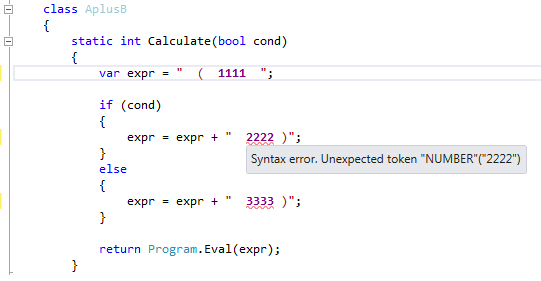
\includegraphics[width=290pt]{picts/Error.png}
%	\end{center}
%\end{frame}

\begin{frame}[fragile]
	\transwipe[direction=90]
	\frametitle{Существующие решения}
	\begin{itemize}
	    \item Alvor -- плагин для Eclipse для статической проверки встроенного в Java SQL
	    \item Java String Analyzer -- статический анализатор динамических выражеинй для Java
		\item PHP String Analyzer -- статический анализатор динамических выражеинй для PHP
        \item PHPStorm -- IDE для PHP с поддержкой HTML, CSS, JavaScript
        \item IntelliLang -- плагин к PHPStorm и IDEA, осуществляющий поддержку различных языков
    \end{itemize}
    %\pause
    \begin{itemize}
        \item Предоставляемая функциональность часто скудна
	    \item Часто поддержка других языков возможна только путём изменения исходного кода инструмента
    \end{itemize}
\end{frame}

\begin{frame}[fragile]
	\transwipe[direction=90]
	\frametitle{Цели}
	\begin{itemize}
	    \item Платформа для создания инструментов анализа встроенных языков
    	\begin{itemize}
    		\item Расширяемость в смысле поддержки других языков
        	\item Расширяемость в смысле предоставляемой функциональности
        \end{itemize}
        \item Плагин для MS Visual Studio на основе ReSharper
    	\begin{itemize}
    		\item Демонстрация возможностей платформы
        	\item Поддержка встроенных языков в MS Visual Studio
        \end{itemize}
    \end{itemize}
\end{frame}

\begin{frame}[fragile]
	\transwipe[direction=90]
	\frametitle{Языковые расширения}
	\begin{itemize}
	    \item Поддержка нового языка -- создание плагина на основе общей функциональности
        \begin{center}
            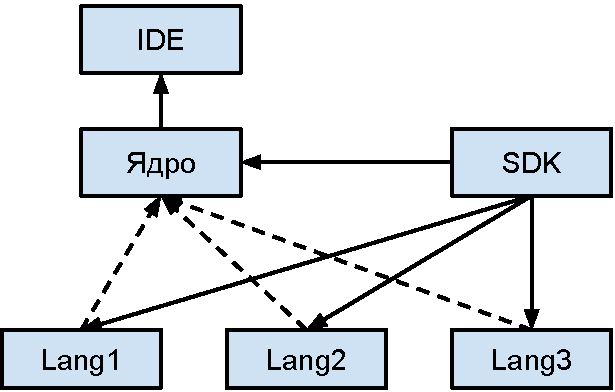
\includegraphics[width=290pt]{picts/Structure.pdf}
        \end{center}
    \end{itemize}
            
\end{frame}

\begin{frame}[fragile]
	\transwipe[direction=90]
	\frametitle{Языковые расширения}
	\begin{itemize}
	    \item SDK
    	\begin{itemize}
    		\item Генератор абстрактных лексических анализаторов
        	\item Генератор абстрактных синтаксических анализаторов
        	\item Описание общих интерфейсов
        	\item ...
        \end{itemize}
	    \item Плагинная система на основе Mono.Addins
	    \item Механизм разметки кода конечного пользователя
    \end{itemize}
\end{frame}

\begin{frame}[fragile]
	\transwipe[direction=90]
	\frametitle{Языковые расширения: пример}
	\begin{Verbatim}[commandchars=\\\{\}]
\textcolor{blue}{var} tbl1 = \textcolor{orange}{“#tbl1”} 
\textcolor{blue}{var} tbl2 = \textcolor{orange}{“tbl2”}

\textbf{[<\textcolor{blue}{InjectedLang}(\textcolor{orange}{"TSQL"})>]}
\textcolor{blue}{execute} (\textcolor{orange}{“select x from ”} + \textcolor{blue}{if} cond \textcolor{blue}{then} tbl1 \textcolor{blue}{else} tbl2)

\textbf{[<\textcolor{blue}{InjectedLang}(\textcolor{orange}{"Calc"})>]}
\textcolor{blue}{eval} (\textcolor{orange}{“12 + 3 * (4 + 5)”})
        \end{Verbatim}
\end{frame}

\begin{frame}[fragile]
	\transwipe[direction=90]
	\frametitle{Как это работает: абстрактный анализ }
	\begin{itemize}
    	\item Kyung-Goo Doh, Hyunha Kim, David A. Schmidt
    	\begin{itemize}
    		\item Комбинация LR-анализа и анализа потока данных для обработки встроенных языков
        \end{itemize}
	    \item Для каждого выражения строится конструкция, аппроксимирующая множество его возможных значений
    	\begin{itemize}
    		\item Data-flow уравнение
        	\item \textbf{Граф}
        	\item Регулярное выражение
        \end{itemize}
	    \item Выполнение лексического, синтаксического анализа над графом
%	    \item Вычисление семантики.
%	    \item ...
    \end{itemize}
\end{frame}

\begin{frame}[fragile]
	\transwipe[direction=90]
	\frametitle{Пример}
		\begin{itemize}
	\item
		\begin{Verbatim}[commandchars=\\\{\}]
\textcolor{blue}{IF} @X = @Y
    \textcolor{blue}{SET} @TABLE = \textcolor{orange}{'#table1'}
\textcolor{blue}{ELSE}
    \textcolor{blue}{SET} @TABLE = \textcolor{orange}{'table2'}
\textcolor{blue}{EXECUTE} 
    (\textcolor{orange}{'SELECT x FROM '} + @TABLE + \textcolor{orange}{' WHERE ISNULL(n,0) > 1'})
		\end{Verbatim}
     	\item Множество значений: \\ \{'SELECT x FROM \#table1 WHERE ISNULL(n,0) > 1' ; \\ \vspace{2pt} 'SELECT x FROM table2 WHERE ISNULL(n,0) > 1'\}
    	\item Аппроксимация: 
            %\begin{center}
                \includegraphics[width = 0.9\textwidth]{picts/approximation1.eps}
            %\end{center}

	\end{itemize}

\end{frame}

\begin{frame}[fragile]
	\transwipe[direction=90]
	\frametitle{Абстрактный лексический анализ}
    \begin{itemize}
    	\item Аппроксикация (граф со строками на рёбрах) $\rightarrow$ граф с токенами на рёбрах
    	\begin{itemize}
    	    \item Привязка к литералу в исходном коде
    	    \item Точная привязка внутри литерала
    	\end{itemize}
    	\item Например:
	    	\begin{itemize}
    	    \item Входной граф
                \begin{center}
                    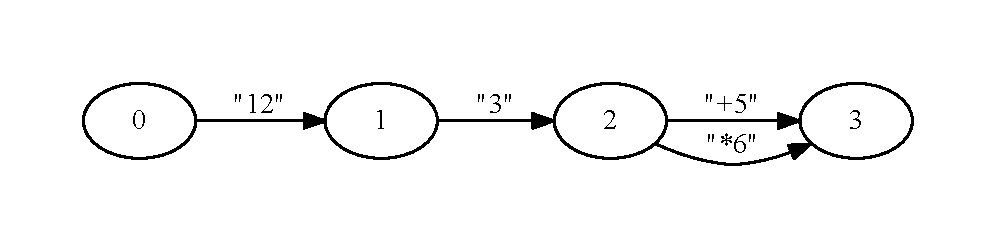
\includegraphics[width=280pt]{picts/example_calc_break.pdf}
                \end{center}
    	    \item Результат лексического анализа
                \begin{center}
                    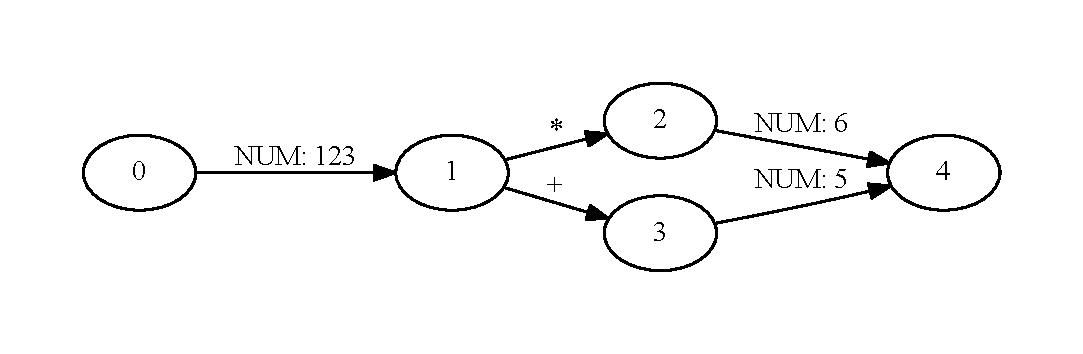
\includegraphics[width=280pt]{picts/res_ex_calc_break.pdf}
                \end{center}
    	\end{itemize}
	\end{itemize}
\end{frame}

\begin{frame}[fragile]
	\transwipe[direction=90]
	\frametitle{Абстрактный лексический анализ: рваные токены}
	\begin{itemize}
    	\item Токены могут собираться из нескольких частей
	        \begin{center}
	            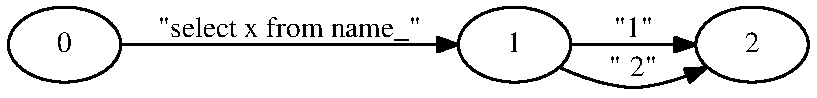
\includegraphics[width=290pt]{picts/brackingLiterals.pdf}
	        \end{center}
    	\item Нужно обрабатывать такие ситуации
    	\item Нужно сохранять привязку каждой части
	\end{itemize}
	
\end{frame}

\begin{frame}[fragile]
	\transwipe[direction=90]
	\frametitle{Обобщённый синтаксический анализ}
    \begin{itemize}
    	\item Generalized LR parsing (GLR)
    	\item Предназначен для работы с произвольными КС грамматиками
	    \begin{itemize}
    	    \item Shift-Reduce и Reduce-Reduce конфликты
    	\end{itemize}
    	\item Использует организованный в виде графа стек (GSS)
	        \begin{center}
	            
\includegraphics[width=250pt]{picts/stack.pdf}
	        \end{center}
    	\item Использует компактное представление леса вывода (SPPF)
	        \begin{itemize}
	            \item Переиспользование общих узлов
	        \end{itemize}
	\end{itemize}
\end{frame}

\begin{frame}[fragile]
	\transwipe[direction=90]
	\frametitle{Абстрактный синтаксический анализ}
     \begin{itemize}
    	\item Добавим Shift-Shift ''конфликты`` -- ситуации, возникающие при ветвлении входного потока
    	\item Получилось расширение GLR
	    \item Вход:
	    \begin{center}
        \begin{dot2tex}[dot]
            digraph G
            {
                rankdir=LR
                d2toptions="--autosize";                    
                0->1[label=" ", texlbl="1"]
                1->2[label=" ", texlbl="+"]
                2->3[label=" ", texlbl="2"]
                2->3[label=" ", texlbl="3"]        
            }
        \end{dot2tex}
	    \end{center}
	    \item Результат: 
	    \begin{center}
	        \begin{tabular}{c | c}
            \begin{dot2tex}[dot]
                digraph G
                {
                    d2toptions="--autosize";
                    0[label="+"]
                    1[label="1"]
                    2[label="2"]
                    0->1
                    0->2
                }
            \end{dot2tex}
            &
            \begin{dot2tex}[dot]
                digraph G
                {
                    d2toptions="--autosize";
                    0[label="+"]
                    1[label="1"]
                    2[label="3"]
                    0->1
                    0->2
                }
            \end{dot2tex}
            \end{tabular}
	    \end{center}
	\end{itemize}
\end{frame}

\begin{frame}[fragile]
	\transwipe[direction=90]
	\frametitle{Диагностика ошибок}
    \begin{itemize}
    	\item Нужно возвращать лес разбора для корректных выражений и список ошибок для некорректных
        \item Для обычного GLR умершая ветка — нормально, для абстрактного не всегда
        \item Пропускать токены в графе сложнее, чем в линейном потоке
	        \begin{center}
	            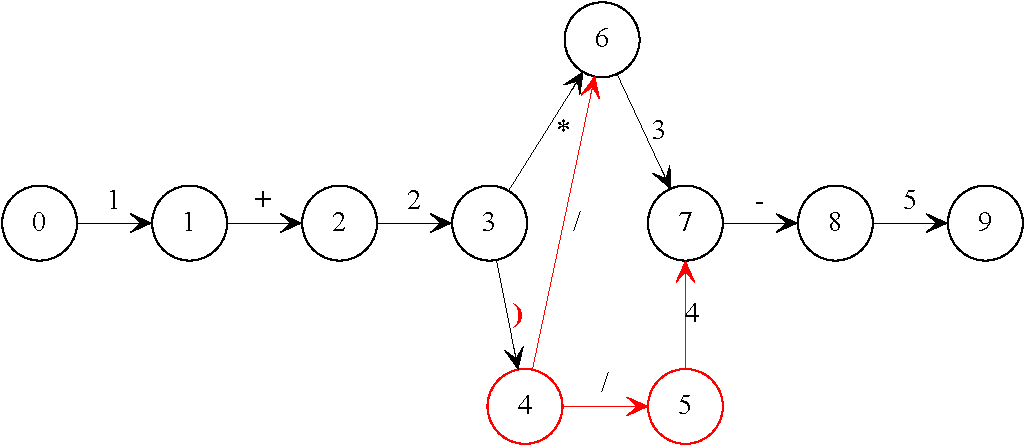
\includegraphics[width=290pt]{picts/IgnoringPaths.pdf}
	        \end{center}
        \item Существуют проблемы, связанные с особенностями базового (GLR) алгоритма
	\end{itemize}
\end{frame}

\begin{frame}[fragile]
	\transwipe[direction=90]
	\frametitle{Восстановление после ошибок}
    \begin{itemize}
        \item Отдельный вопрос для исследований
        \begin{itemize}
            \item В больших выражениях хочется видеть все ошибки
            \item В сложных выражениях может быть много ложных ошибок
            \item Бывают принципиально некорректные выражения, которые при реальном выполнении не формируются
            \item Например
            
            \begin{Verbatim}[commandchars=\\\{\}]
            x = condition ? \textcolor{orange}{“(1+2”} : \textcolor{orange}{“1+2”};
            y = condition ? \textcolor{orange}{“)*3”} : \textcolor{orange}{“*3”};
            Program.Eval(x + y);
            \end{Verbatim}
            2 из 4 путей не могут быть получены, но в графе есть все
	        \begin{center}
	            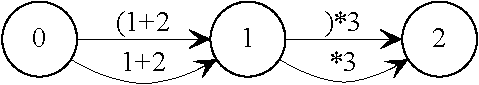
\includegraphics[width=200pt]{picts/4insteadOf2.pdf}
	        \end{center}
        \end{itemize}
	\end{itemize}
\end{frame}

\begin{frame}[fragile]
	\transwipe[direction=90]
	\frametitle{Вычисление семантики}
    \begin{itemize}
        \item Результат анализа -- минимум одно дерево для пути в графе и весь лес разбора сжат в SPPF
        \item Что-то можно вычислить прямо на графе, но часто нужно извлекать деревья
    \end{itemize}
    
    \begin{figure}[h]
        \begin{subfigure}[h]{0.33\textwidth}
            \includegraphics[width=40pt]{picts/before_tokenization.eps}
        \end{subfigure}
        \qquad \qquad
        \begin{subfigure}[h]{0.33\textwidth}
            \includegraphics[width=135pt]{picts/Calc_sppf.eps}
        \end{subfigure}
    \end{figure}
\end{frame}


\begin{frame}[fragile]
	\transwipe[direction=90]
	\frametitle{Вычисление семантики: пример}
    Подсветка синтаксиса
    \begin{itemize}
        \item Достаточно покрыть все токены
        \item Можно возвращать не все деревья, а некоторое подмножество
        \begin{center}
            \includegraphics[width=290pt]{picts/idea1_input.eps}
        \end{center}
    \end{itemize}
    \begin{figure}[h]
        \begin{subfigure}[h]{0.33\textwidth}
            \includegraphics[width=120pt]{picts/idea1_tree1_light.eps}
        \end{subfigure}
        \qquad \qquad
        \begin{subfigure}[h]{0.33\textwidth}
            \includegraphics[width=120pt]{picts/idea1_tree2_light.eps}
        \end{subfigure}
    \end{figure}
    
\end{frame}

\begin{frame}[fragile]
	\transwipe[direction=90]
	\frametitle{Вычисление семантики}
    \begin{itemize}
        \item В худшем случае придётся перебирать все деревья
        \begin{center}
            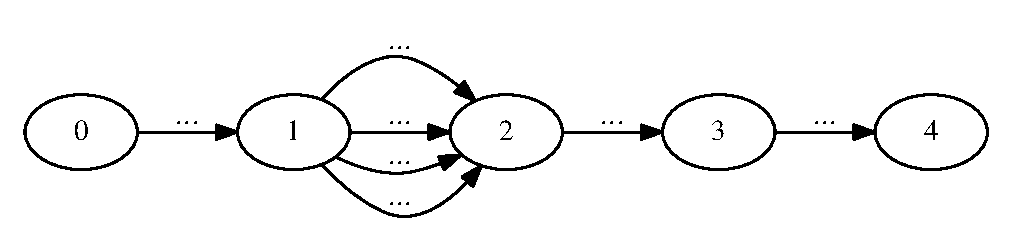
\includegraphics[width=290pt]{picts/Bad_case.eps}
        \end{center}
        \item Ленивая генерация деревьев
    \end{itemize}
\end{frame}

\begin{frame}[fragile]
	\transwipe[direction=90]
	\frametitle{Демонстрация}
		\begin{center}
		    \animategraphics[autoplay,loop,height=7.5cm]{13}{picts/BigSample/frame_}{001}{334}
		\end{center}
\end{frame}

\begin{frame}[fragile]
	\transwipe[direction=90]
	\frametitle{Что дальше}
	\begin{itemize}
        \item Большинство задач, применимых к обычному коду, применимо и ко встроенным языкам:
        \begin{itemize}
            \item навигация
            \item проверка типов
            \item трансформации
            \item ...
        \end{itemize}
        %\pause
        %\item Что-то в планах. Над чем-то уже работаем.
	\end{itemize}
\end{frame}


\begin{frame}[fragile]
	\transwipe[direction=90]
	\frametitle{Навигация по коду}
	\begin{itemize}
        \item Визуальное представление динамического выражения в виде графа
        \begin{itemize}
            \item Навигация в код
            \item Навигация в граф из кода
            \item Информация об ошибках на графе: если ошибка на стыке строковых литералов, то трудно понять, где она реально
        \end{itemize}
	\end{itemize}
	\begin{center}
            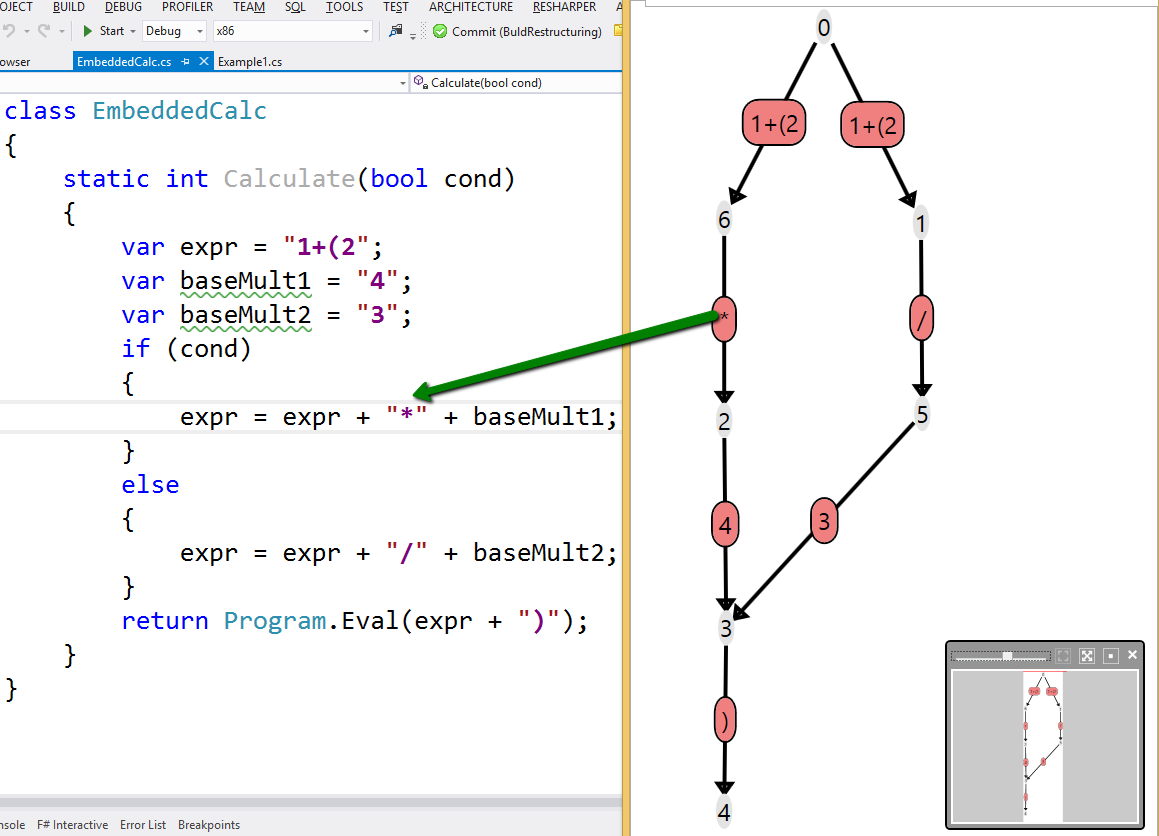
\includegraphics[width=290pt]{picts/Navigate2.png}
        \end{center}
\end{frame}

\begin{frame}[fragile]
	\transwipe[direction=90]
	\frametitle{Проверка типов}
	\begin{itemize}
        \item Внутри выражения
        \begin{itemize}
            \item 
                \begin{Verbatim}[commandchars=\\\{\}]
    \textcolor{blue}{int} x = \textcolor{blue}{eval} (\textcolor{orange}{“12 * 'string' + 3 ”})
                \end{Verbatim}
        \end{itemize}
		\item Согласованность с внешним кодом
    	\begin{itemize}
            \item 
                \begin{Verbatim}[commandchars=\\\{\}]
    \textcolor{blue}{int} x = \textcolor{blue}{execute} (\textcolor{orange}{“select 'string' from dual”})
                \end{Verbatim}
        \end{itemize}
	\end{itemize}
\end{frame}


\begin{frame}
	\transwipe[direction=90]
	\frametitle{Трансформации}
	\begin{itemize}
        \item Рефакторинг
		\item Переход с одного диалекта на другой
    	\begin{itemize}
            \item Для SQL особенно актуально
        \end{itemize}
        \item Переход на новые технологии
    	\begin{itemize}
            \item Встроенный SQL $\rightarrow$ LINQ
        \end{itemize}
	\end{itemize}
    Много вопросов
	\begin{itemize}
		\item Возможны ли нетривиальные трансформации?
    	\begin{itemize}
            \item Как обратно генерировать код?
        \end{itemize}

		\item Как гарантировань корректность трансформаций?
	\end{itemize}
\end{frame}

\begin{frame}[fragile]
	\transwipe[direction=90]
	\frametitle{Результаты}
	\begin{itemize}
	    \item Ядро
	    \begin{itemize}
	        \item Генератор абстрактных лексических анализаторов
    	    \begin{itemize}
                \item Привязка к исходному коду
	        \end{itemize}
	        \item Генератор абстрактных синтаксических анализаторов
    	    \begin{itemize}
                \item Диагностика ошибок
                \item Механизм вычисления семантики
	        \end{itemize}
            \item Модульная архитектура для языковых расширений
        \end{itemize}
	    \item Плагин для ReSharper
	    \begin{itemize}
	        \item Расширяемая архитектура, позволяющая легко поддержать любой встроенный язык
	        \begin{itemize}
	            \item Внешний язык должен поддерживаться в ReSharper
            \end{itemize}
        \end{itemize}
	\end{itemize}
\end{frame}

\begin{frame}[fragile]
	\transwipe[direction=90]
	\frametitle{Реализация}
	\begin{itemize}
	    \item Открытый код
	    \item Платформа .NE.
	    \item Основной язык -- F\#
	    \item Проект YaccConstructor -- платформа для исследований в области синтаксического анализа
	\end{itemize}
\end{frame}

\begin{frame}
	\transwipe[direction=90]
	\frametitle{Область применения}
	\begin{itemize}
		\item Поддержка встроенных языков в IDE
    	\begin{itemize}
            \item Интерактивная ("на лету")
            \item "Офлайновая" \ проверка (ручной запуск)
        \end{itemize}
        \item Поддержка, сопровождение кода со встроенными языками
		\item Автоматизированный реинжиниринг ПО, разработанного с применением встроенных языков
		\item Верификация генераторов кода
	\end{itemize}
\end{frame}

\begin{frame}
	\transwipe[direction=90]
	\frametitle{Информация о проекте}
	\begin{itemize}
		\item Контакты: 
        \begin{itemize}
            \item Григорьев Семён: Semen.Grigorev@jetbrains.com
            \item Вербицкая Екатерина: kajigor@gmail.com
            \item Мавчун Екатерина: emavchun@gmail.com
            \item Иванов Андрей: ivanovandrew2004@gmail.com
            \item Полубелова Марина: polubelovam@gmail.com
        \end{itemize}
		\item Исходный код YaccConstructor: \href{http://recursive-ascent.googlecode.com}{http://recursive-ascent.googlecode.com}
		\item Google+ сообщество: \href{https://plus.google.com/u/0/communities/102842370317111619055}{https://plus.google.com/u/0/communities/102842370317111619055}
		\item Сообщество GitHub: \href{https://github.com/YaccConstructor}{https://github.com/YaccConstructor}
	\end{itemize}
\end{frame}

\end{document}
